\begin{exo}
	Soient $A$, $B$, et $C$, trois points dans le repère $\OIJ$ ci-dessous. Les affirmations suivantes sont-elles vraies ou fausses ? Justifier.
	\begin{center}
		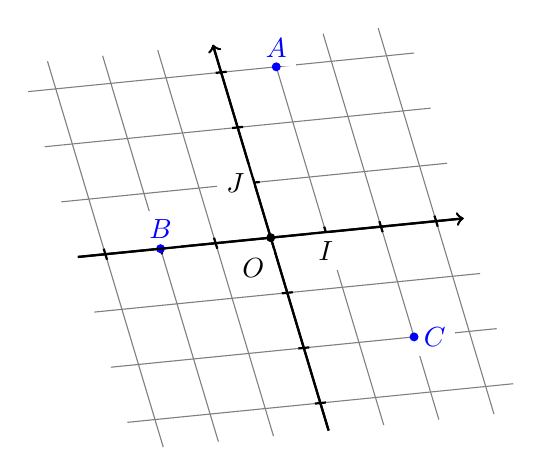
\begin{tikzpicture}[scale=0.7, x={(1cm, 0.1cm)}, y={(-0.3cm, 1cm)}]
			\draw[thick,->] (-3.5,0) -- (3.5,0); \draw[thick,->] (0,-3.5) -- (0,3.5);
			\foreach \x in {-3,-2,-1,1,2,3} { \draw[gray, thin] (\x, -3.5) -- (\x, 3.5); \draw[thick] (\x, -0.1) -- (\x, 0.1); }
			\foreach \y in {-3,-2,-1,1,2,3} { \draw[gray,thin] (-3.5,\y) -- (3.5,\y); \draw[thick] (-0.1,\y) -- (0.1,\y); }
			\node at (0,-0.2) [below left, fill=white] {$O$};
			\node at (1,0) [below, fill=white] {$I$};
			\node at (0,1) [left, fill=white] {$J$};
			\coordinate (A) at (1,3);
			\coordinate (B) at (-2,0);
			\coordinate (C) at (2,-2);
			\foreach \p/\name/\pos in {A/A/above, B/B/above, C/C/right} {
					\node[\pos, blue, fill=white] at (\p) {$\name$};
					\filldraw[blue] (\p) circle (2pt);
				}
			\draw[thick,->] (-3.5,0) -- (3.5,0); \draw[thick,->] (0,-3.5) -- (0,3.5);
			\filldraw (0,0) circle (2pt);
		\end{tikzpicture}
	\end{center}
	\begin{enumerate}
		\item Le repère $\OIJ$ est un repère orthogonal.
		\item L'abscisse du point $A$ est égale à $1$.
		\item L'ordonnée du point $B$ est égale à $0$.
		\item Le point $C$ a pour coordonnées $\coordl{-2}{2}$.
	\end{enumerate}
\end{exo}
